\documentclass[aspectratio=169,xcolor=usenames,dvipsnames,svgnames]{beamer}

\usepackage{fontspec}
\usepackage{appendixnumberbeamer}
\usepackage{tikz}
\usepackage{varwidth}
\usepackage{pstricks}
\usepackage{polyglossia}
\usepackage{csquotes}
\usepackage{xsavebox}
\usepackage{pifont}
\usepackage{xurl}
\usepackage[style=authoryear]{biblatex}
\usepackage{pgfplots}
%\usepackage[shortlabels]{enumitem}

\setmainlanguage{german}
\MakeOuterQuote{"}

\usetheme[numbering=fraction]{metropolis}
\setsansfont[BoldFont={Fira Sans SemiBold}]{Fira Sans Book}
\metroset{block=fill}

\usetikzlibrary{patterns}
\usetikzlibrary{shapes}
\usetikzlibrary{shapes.symbols}
\usetikzlibrary{positioning}
\usetikzlibrary{fit}
\usetikzlibrary{backgrounds}
\usetikzlibrary{calc}

\pgfplotsset{compat=1.16}
\usepgfplotslibrary[dateplot]

\newcommand{\tikzdbg}{%
  \draw[step=1,color=lightgray] (-7,0) grid (10,10);%
  \fill[red] (0,0) circle (0.2);%
}

\tikzset{
  onslide/.code args={<#1>#2}{%
    \only<#1>{\pgfkeysalso{#2}}% \pgfkeysalso doesn't change the path
  },
  temporal/.code args={<#1>#2#3#4}{%
    \temporal<#1>{\pgfkeysalso{#2}}{\pgfkeysalso{#3}}{\pgfkeysalso{#4}}%
  },
  hidden/.style = {opacity=0},
  uncover/.style = {temporal=#1{hidden}{}{hidden}},
  drawalert/.style = {temporal=#1{}{color=alerted text.fg}{}}
}

\colorlet{pgreen}{OliveGreen}
\colorlet{pplum}{black!50!Plum}
\colorlet{pblue}{Cyan}
\colorlet{pdim}{black!10}


\newenvironment{tikzcomponent}[1]{%
  \begin{xlrbox}{#1}%
    \begin{tikzpicture}%
    }{
    \end{tikzpicture}%
  \end{xlrbox}%
}

\newcommand{\TODO}[1]{
  \red{TODO: #1}
}

\bibliography{./bib-refs.bib}

\typeout{CONTENT START NOW}

\title{Generierung angepasster RDF-Dumps von Wikidata}
\subtitle{Bachelorverteidigung}
\date{16. Januar 2020}
\author{Benno Fünfstück}
\institute{Betreuer: Prof. Dr. Markus Krötzsch \\ Wissensbasierte Systeme \\ TU Dresden}

\begin{document}

%\includeonlyframes{first,current}
    
\begin{frame}[label=first]
  % gear symbol
\begin{tikzcomponent}{gear}
  \foreach \angle in {0, 60, ..., 360} {
    \draw[fill=black] (0,0) -- (\angle-30:0.7cm) -- (\angle-30+8:0.7cm) -- (\angle-13:1cm) -- (\angle+13:1cm) -- (\angle+30-8:0.7cm) -- (\angle+30:0.7cm) -- cycle;
  };
  \draw[fill=white] (0,0) circle [radius=0.3];
\end{tikzcomponent}

% database symbol
\begin{tikzcomponent}{database}
  \pgfmathsetmacro{\radius}{0.8};
  \begin{scope}[line width=1pt]
    \draw (0,0) circle [x radius=\radius, y radius=0.3];
    \draw (-\radius,0) -- (-\radius,-1.5);
    \draw (\radius,0) -- (\radius,-1.5);
    \draw (-\radius,-0.5) arc[start angle=180, delta angle=180, x radius=\radius, y radius=0.3];
    \draw (-\radius,-1.0) arc[start angle=180, delta angle=180, x radius=\radius, y radius=0.3];
    \draw (-\radius,-1.5) arc[start angle=180, delta angle=180, x radius=\radius, y radius=0.3];
  \end{scope};
\end{tikzcomponent}

% web server symbol
\begin{tikzcomponent}{webserver}
  \begin{scope}[scale=1.2]
    \pgfmathsetmacro{\frontwidth}{1};
    \pgfmathsetmacro{\backwidth}{0.6};
    \pgfmathsetmacro{\topheight}{0.5};
    \draw[fill=black] (-\backwidth, 0) -- (\backwidth,0) -- (\frontwidth,-\topheight) -- (-\frontwidth,-\topheight) -- cycle;
    \draw[fill=black] (-1.1\frontwidth, -\topheight-0.1) rectangle (1.05\frontwidth, -\topheight-0.6);
    \foreach \i in {0,1,2} {
      \draw[fill=white] (\frontwidth*\i/3+0.15\frontwidth, -\topheight-0.35) circle [radius=1mm];
    }
  \end{scope}
\end{tikzcomponent}

% archive symbol
\begin{tikzcomponent}{archive}
  \begin{scope}[line width=1pt]
    \pgfmathsetmacro{\width}{1.8};
    \pgfmathsetmacro{\shear}{0.8};
    \pgfmathsetmacro{\topheight}{0.6};
    \pgfmathsetmacro{\gap}{0.2};
    \draw (0,0) rectangle (\width,-1);
    \draw (0,0) rectangle (\width,\gap);
    \draw (0,\gap) -- ({(1-\shear)*\width},\gap+\topheight) -- (\width*\shear,\gap+\topheight) -- (\width,0.2) -- cycle;
    \node[rectangle, draw, rounded corners=4pt, inner xsep=8pt] at (0.5*\width,-0.5) {};
  \end{scope}
\end{tikzcomponent}

% client pc symbol
\begin{tikzcomponent}{client}
  \draw [line width=3mm] (0,0) rectangle (2,1.3);
  \draw [line width=2mm] (0,-0.4) -- (2, -0.4);
\end{tikzcomponent}

  \maketitle
\end{frame}

\setbeamertemplate{frame footer}[custom]{%
  Bachelorverteidigung: \insertshortauthor
}

\begin{frame}
  \centering
  
\includegraphics[width=0.6\textwidth]{./pics/Wikidata-logo-en} \\
  "Die freie Wissensdatenbank mit 74.018.298 Datensätzen, die jeder bearbeiten kann."
\end{frame}

\begin{frame}\frametitle{Wikidata: Items}
  \centering
  \begin{tikzpicture}
  \coordinate (base) at (1.5, 1.5);

  \node[above=7pt of base, anchor=south west, inner sep=0pt] (label) {\Large{Douglas Adams}};
  \node[color=black!70, right=5pt of label] (id) {(Q42)};

  \draw (base) -- +(7, 0) coordinate (lineend);

  \node[below=8pt of base, anchor=north west, inner sep=0pt] (description) {britischer Schriftsteller (1952-2001)};
  \node[color=black!70, below=23pt of base, inner sep=0pt, anchor=north west] (aliases) {Douglas Noël Adams | Douglas Noel Adams};

  \coordinate[below=45pt of base] (linkbase);

  \draw[fill, color=blue] (linkbase) ++(5pt,0) -- ++(0,-6pt) -- ++(4pt, 3pt)
  node[anchor=west] (link) {In weiteren Sprachen};

  \node[below=65pt of base, anchor=north west] (statements) {\large{Statements}};
  \node[below=85pt of base, anchor=north west] (statements) {\large{Sitelinks}};

  \node[draw, fit=(label) (id) (link) (lineend) (aliases) (statements), inner sep=10pt] {};

  % labels
  \draw[dashed] (2,3.5) node[anchor=south] {label} -- (label);
  \draw[dashed] (6,3.5) node[anchor=south] {item identifier} -- (id);
  \draw[dashed] (10,0 |- description)  node[anchor=west] {description} -- (description);
  \draw[dashed] (10,0  |- aliases) node[anchor=west] {aliases} -- (aliases);
\end{tikzpicture}

\end{frame}

\begin{frame}\frametitle{Wikidata: Statements}
  \centering
  \begin{tikzpicture}
  \node[anchor=west, color=pgreen] (snak1title) {St John's College \small (Q691283)};
  \coordinate[below=13pt of snak1title.north west] (snak1bot);
  \matrix[xshift=10pt, matrix anchor=north west, every cell={anchor=west}] (snak1quals) at (snak1bot) {
    \node[anchor=west] {start time \small{(P580)}}; & \node (qual1) {1971}; \\
    \node[anchor=west] {end time \small{(P582)}}; & \node (qual2) {1974}; \\
  };
  \coordinate (snak1end) at (snak1title.west |- snak1quals.south);
  \node[fit=(snak1title) (snak1quals)] (snak1) {};

  \coordinate[below=5pt of snak1end] (snak2corner);
  \node[anchor=north west, color=pgreen] (snak2title) at (snak2corner) {Brentwood School \small (Q4961791)};
  \coordinate[below=13pt of snak2title.north west] (snak2bot);
  \matrix[xshift=10pt, matrix anchor=north west, every cell={anchor=west}] (snak2quals) at (snak2bot) {
    \node[anchor=west, xshift=10pt] {start time \small{(P580)}}; & \node{1959}; \\
    \node[anchor=west, xshift=10pt] {end time \small{(P582)}}; & \node{1970}; \\
  };
  \node[fit=(snak2title) (snak2quals)] (snak2) {};

  \node[left=7pt of snak1.north west, color=pplum, anchor=north east, inner sep=5pt, align=left] (property) {educated at \\ \small{(P69)}};
  \begin{scope}[on background layer]
    \fill[color=pdim] (property.east |- snak1.north) rectangle (property.west |- snak2.south);
  \end{scope}
  \node[draw, very thick, fit=(property) (snak1) (snak2), inner sep=0pt] (frame) {};


  % Labels
  \begin{scope}[thick]
    \node[above=15pt of property, color=pplum] (proplabel) {Property};
    \draw[dashed, color=pplum] (proplabel) -- (property);

    \node[right=25pt of snak1title.east, color=pgreen] (valuelabel) {Value};
    \draw[dashed, color=pgreen] (valuelabel) -- (snak1title);

    \coordinate (join) at ($(qual1.east)!0.5!(qual2.east)$);
    \draw[dashed] (qual1.east) -- (qual2.east) (join) -- (valuelabel.west |- join) node[anchor=west] {Qualifier};

    \node[below=2pt of frame] {\textbf{Statement Group}};
  \end{scope}

  %\node[anchor=west, color=pgreen, below=of snak1.south east]{};
  % \matrix[anchor=west, every cell={width=20pt}] at (snak2pos) {
  % };
\end{tikzpicture}

\end{frame}


\section{Idee: Tool zum Filtern der Daten}

% \begin{frame}[fragile]\frametitle{Beispiele}
%   GraFa: Faceted Search \& Browsing for the Wikidata Knowledge Graph \\
%   (\cite{usage-grafa}) \\
% nur "truthy" Statements mit Entitäten als Objekt;
%   Labels/Descriptions nur in Englisch und Spanisch \\
%   \vspace{0.5cm}

%   Populating Narratives Using Wikidata Events: An Initial Experiment \\
%   (\cite{usage-narratives}) \\
%   alle  Items mit einem Statement für mindestens eine von 50 festgelegten
%   Properties
% \end{frame}

\begin{frame}{Anforderungen}
  \alert{\textbf{Filterung:}} Einen Dump aus einer Teilmenge der Daten erzeugen, nach
  nutzerdefinierten \emph{Kriterien}

  Diese Dumps sollen \textbf{archiviert} werden und das Archiv \textbf{durchsuchbar} sein.

  \pause

  Anforderungen an das Interface:
  \begin{itemize}
      \item Prozess ist \textbf{nachvollziehbar}: Ursprung, Inhalt des Dumps
      \item Feedback zu \textbf{Fortschritt}
      \item mehrere Nutzer können parallel Dumps erzeugen (\textbf{Parallelverarbeitung})
  \end{itemize}

  \pause

  Format der Dumps: \emph{RDF (Resource Description Framework)}
\end{frame}


\begin{frame}[label=current]\frametitle{Filterkriterien}
  Konzeptionell drei Ebenen:
  \begin{itemize}
    \item Auswahl der Items
    \item Auswahl der Statements
    \item Kodierung des Statements
  \end{itemize}

  Unabhängig davon: Labels, Descriptions, Aliases, Sitelinks, Sprache von Literalen
\end{frame}


\begin{frame}[t, fragile]\frametitle{Wikidata als RDF}
  \begin{block}{Tripel für Labels}
  \begin{verbatim}
 wd:Q42 rdfs:label "Douglas Adams"@en .
 wd:Q42 rdfs:label "Douglas Adams"@de .
  \end{verbatim}
    \vspace{-0.2cm}
  \end{block}

  \begin{block}{Einfache Darstellung: ein Tripel für jedes Statement}
  \begin{verbatim}
 wd:Q42 wdt:P69 wd:Q691283 .
 wd:Q42 wdt:P69 wd:Q4961791.
  \end{verbatim}
    \vspace{-0.2cm}
  \end{block}

  \textbf{Aber:} Ranks, Qualifier, Komplexe Werte?
  %\footnotesize{\verb|wd:Q42| ist kurz für \verb|<http://www.wikidata.org/entity/Q42>|}
\end{frame}

\begin{frame}[t, fragile]\frametitle{Wikidata als RDF: Reifikation}
  \vspace{-0.15cm}
  \begin{tikzpicture}[
  n/.style = {draw, rectangle, rounded corners=8pt, minimum height=1cm, font=\small},
  nw/.style = {n, anchor=west},
  e/.style = {->, line width=1pt},
  ]

  \node[n] (q42) at (-1, -1) { wd:Q42 };
  \node[n] (t) at (-1, 2) { wd:Q4961791 };
  \draw[e] (q42) to node[right] {wdt:P69} (t);

  \begin{scope}[uncover=<2->]
    \node[n] (s) at (3, 0) { wds:q42-xxxx };
    \node[nw] (typ) at (6, 0) { wikibase:Statement };

    \draw[e] (q42) to node[above] {p:P69} (s);
    \draw[e] (s) to node[above, outer sep=2pt] {rdf:type} (typ);
    \draw[e] (s) to [bend left=8] node [sloped, above, outer sep=1pt] {ps:P69} (t);
  \end{scope}

  \begin{scope}[uncover=<3->]
    \node[nw] (vn1) at (6.5, 1.5) { wdv:aaaaaaaa };
    \node[nw] (v1) at (0, 3) {\verb|"1959-01-01T00:00:00Z"^^xds:dateTime| };
    \node[nw] (vn2) at (6.5, -1.5) { wdv:bbbbbbbb };
    \node[nw] (v2) at (0, -3) {\verb|"1970-01-01T00:00:00Z"^^xsd:dateTime| };

    \draw[e] (s.south) to node[left, outer sep=2pt] {pq:P582} (v2.north);
    \draw[e] (s) to node [sloped, below, outer sep=1pt] {pqv:P582} (vn2.west);
    \draw[e] (s) to node [sloped, above, outer sep=1pt] {pqv:P580} (vn1.west);
    \draw[e] (s) to node [left, outer sep=1pt] {pq:P580} (v1.south);
  \end{scope}

\end{tikzpicture}

\end{frame}

% \begin{frame}[t, fragile]\frametitle{Wikidata als RDF: Reifikation}
%   \vspace{0.25cm}
%   \begin{block}{RDF}
%   \begin{verbatim}
%  wd:Q42 p:P69 wds:q42-xxxx .
%  wds:Q42-xxxx rdf:type wikibase:Statement .
%  wds:Q42-xxxx ps:P69 wd:Q4961791 .
%  wds:Q42-xxxx pq:P580 "1959-01-01T00:00:00Z"^^xds:dateTime .
%  wds:Q42-xxxx pqv:P580 wdv:aaaaaaaa .
%  wds:Q42-xxxx pq:P582 "1970-01-01T00:00:00Z"^^xsd:dateTime .
%  wds:Q42-xxxx pqv:P582 wdv:bbbbbbbb .
%  wd:Q42 wdt:P69 wd:Q4961791.
%   \end{verbatim}
%   \end{block}
% \end{frame}

\section{Umsetzung}

\begin{frame}\frametitle{Ansatz: Wikidata Query Service}
  \emph{Wikidata Query Service} indiziert den RDF-Export von Wikidata und
  beantwortet SPARQL-Abfragen über diesen Datensatz.

  \textbf{Vorteile:}
  \begin{itemize}
    \item Kann einige Abfragen sehr schnell beantworten
    \item Verwendet aktuelle Daten
  \end{itemize}
  \textbf{Nachteile:}
  \begin{itemize}
    \item Große Dumps führen zu Timeout
    \item Formulierung der Filter in SPARQL umständlich
  \end{itemize}

\end{frame}

\begin{frame}\frametitle{Ansatz: Wikidata Toolkit}
  \emph{Wikidata Toolkit} ist eine Java-Bibliothek zum Verarbeiten der JSON-Exporte von Wikidata.
  \begin{itemize}
      \item Implementiert das RDF Dump Format
      \item Wird aktiv entwickelt
  \end{itemize}

  \textbf{Vorteile:}
  \begin{itemize}
    \item Kann auch sehr große Dumps erzeugen
    \item Filter können in Java geschrieben werden

  \end{itemize}

  \textbf{Nachteile:}
  \begin{itemize}
      \item Langsamer als index-basierte Methoden
      \item Verwendet nicht den "offiziellen" RDF-Export von Wikidata
  \end{itemize}


\end{frame}

\begin{frame}\frametitle{System}
  \begin{figure}
    \begin{tikzpicture}[
  line width=2pt,
  ]
  \node (frontend) at (6.5,0) {\thewebserver};
  \node[below of=frontend, node distance=1.05cm, outer ysep=0.15cm] (frontendtext) {Frontend};

  \node (database) at (2.4,-3) {\thedatabase};
  \node[below of=database, node distance=1.5cm] (databasetext) {Datenbank};
  %\node[below of=databasetext, anchor=north, node distance=0.3cm] {\small Speicherung von Dump-Metadaten};

  \draw[<->] (frontendtext) -- (database);

  \node (backend) at (-2,0) {\thegear};
  \node[drawalert=<4>, below of=backend, anchor=north, node distance=0.9cm,
  align=center, outer ysep=0.2cm] (backendtitle) {Backend};
  %\node[below of=backendtitle, anchor=north, align=left, node distance=0.3cm] (backenddesc) {{\small Verarbeitet regelmäßig Aufträge} \\ {\small aus der Warteschlange}};
  
  \node[line width=1pt, cylinder, draw, shape aspect=0.4, inner ysep=0.3cm, drawalert=<3>] at ($(backend)!0.47!(frontend)$) (queue) { Warteschlange };

  \node (client) at (7,-4) {\theclient};
  \node[below of=client, anchor=north, node distance=1.2cm] (clienttext) { Client };
  \draw[<->,drawalert=<2>] (frontendtext) -- (client);

  \draw[->] ($(frontend.west)+(0.05,0)$) -- ($(queue.east)-(0.25,0)$);
  \draw[->] (queue) -- (backend);

  \draw[->, drawalert=<4>] (backendtitle) to [bend right=10] (database);
  %\draw[->] (backendtitle) to [bend right=10] node[anchor=north east, align=left]{{\small
  %    Aktualisierung}\\ {\small der Dump-Metadaten}} (database);

  \node (zenodo) at (-2,-4) {\thearchive};
  \node[below of=zenodo, anchor=north, node distance=1.0cm] (zenodotext) {Zenodo};
  \draw[drawalert=<5>, ->] (backendtitle) -- (zenodo);
\end{tikzpicture}

  \end{figure}
\end{frame}

\begin{frame}[plain, fragile]
  \centering
  \begin{columns}
    \begin{column}{0.65\framewidth}
      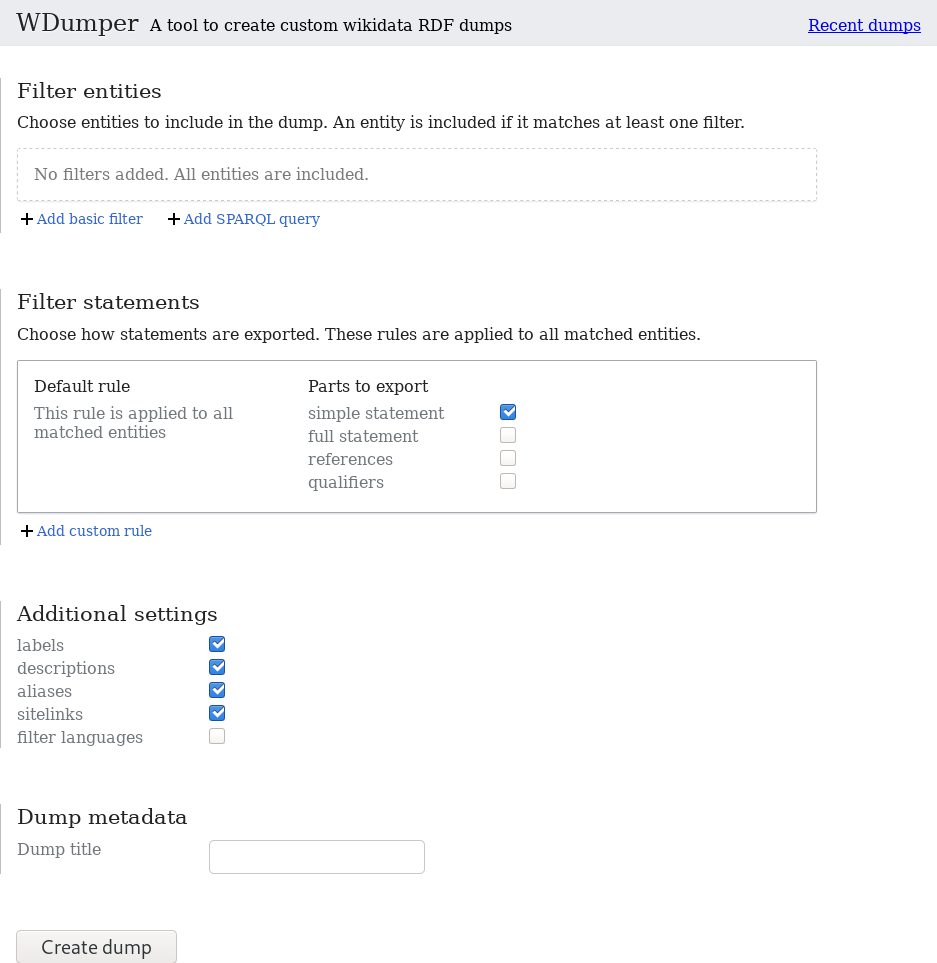
\includegraphics[width=0.65\framewidth]{./pics/screen-main}
    \end{column}
    \begin{column}{0.35\framewidth}
      Deployment auf Toolforge \\
      \vspace{0.5cm}
      Backend in Java \\
      \vspace{0.5cm}
      Frontend in Python/TypeScript \\
      \vspace{0.5cm}
      MariaDB als Datenbank \\
      \vspace{0.5cm}
      \hspace{-110pt}
      \color{blue!80!black}{\url{https://tools.wmflabs.org/wdumps}}
    \end{column}
  \end{columns}
\end{frame}

\section{Evaluation}

\begin{frame}[t]
  \only<1>{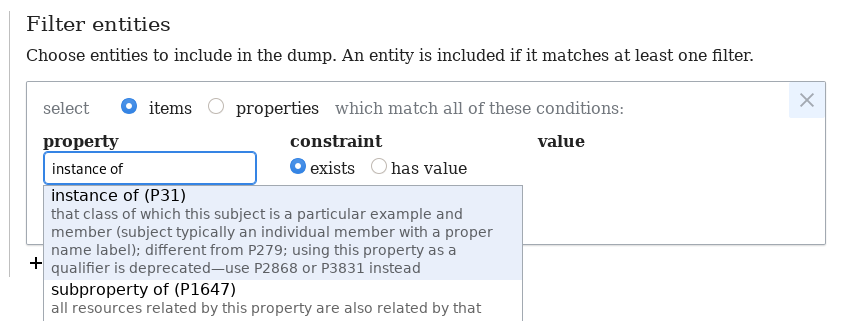
\includegraphics[width=\framewidth]{./pics/uiwalk/1.png}}
  \only<2>{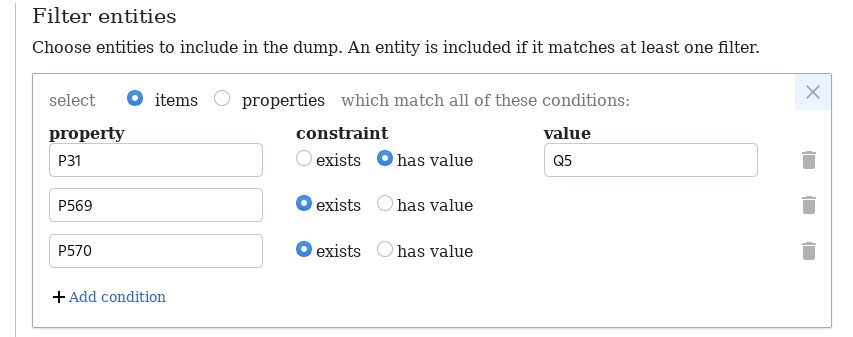
\includegraphics[width=\framewidth]{./pics/uiwalk/2.png}}
  \only<3>{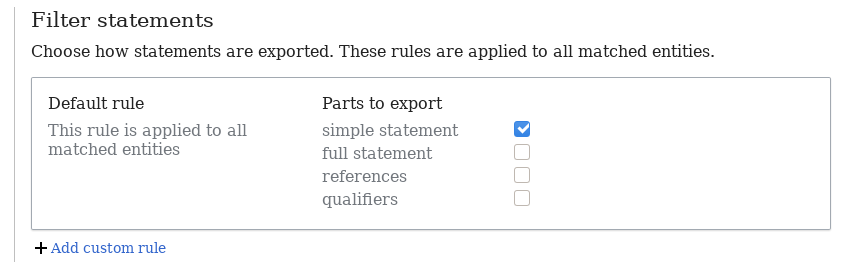
\includegraphics[width=\framewidth]{./pics/uiwalk/3.png}}
  \only<4>{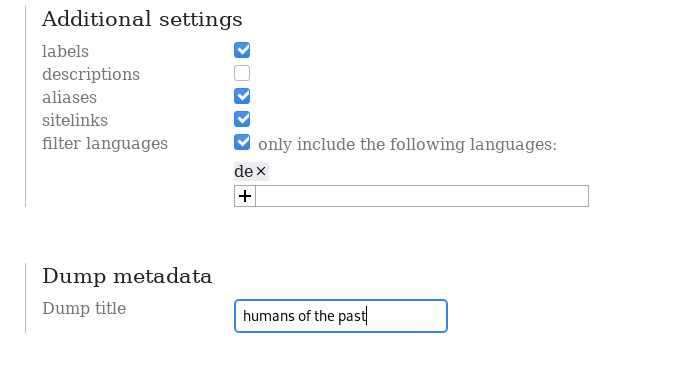
\includegraphics[width=\framewidth]{./pics/uiwalk/5.png}}
  \only<5>{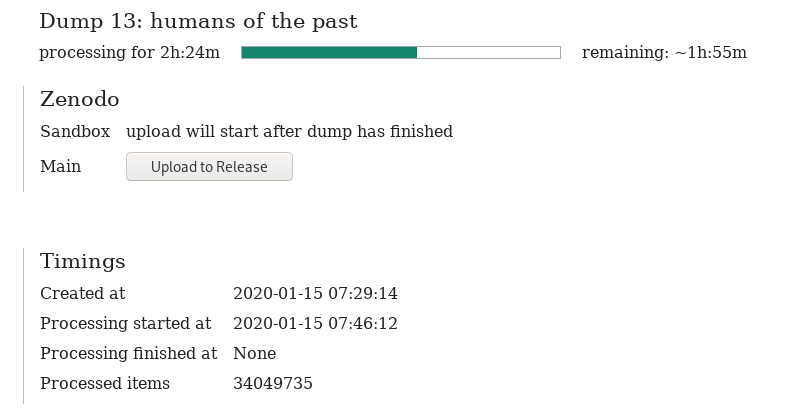
\includegraphics[width=\framewidth]{./pics/uiwalk/6.png}}
  \only<6>{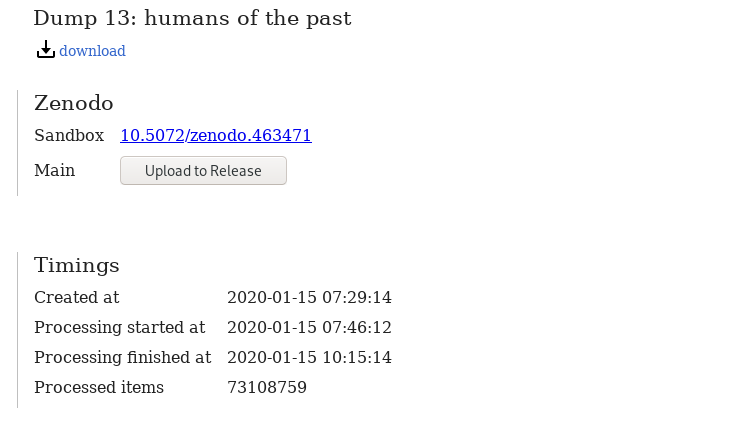
\includegraphics[width=\framewidth]{./pics/uiwalk/7.png}}
  \only<7>{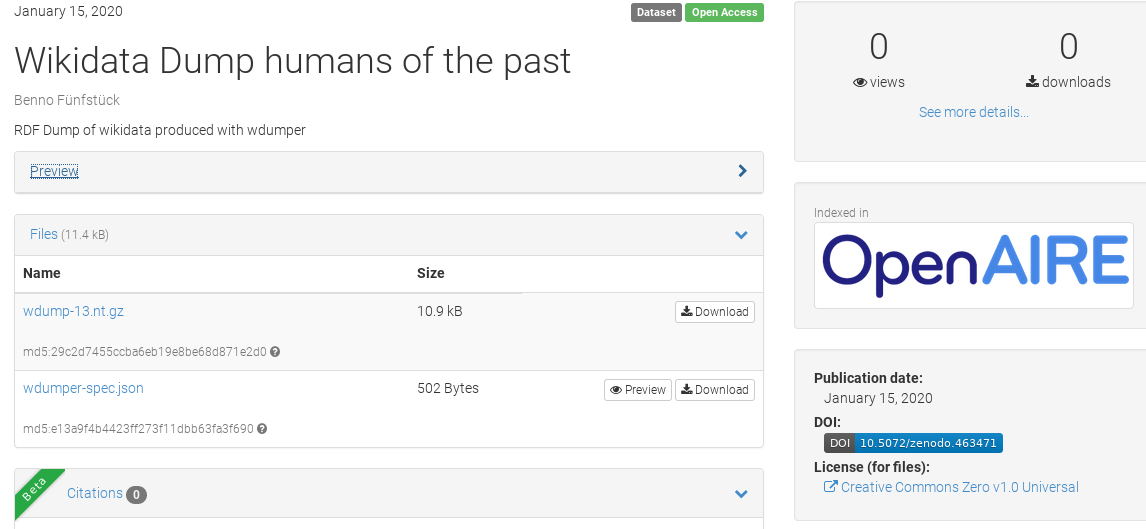
\includegraphics[width=\framewidth]{./pics/uiwalk/8.png}}
\end{frame}

\begin{frame}\frametitle{Korrektheit}
  Die Anwendung verwendet Wikidata Toolkit zur Generierung der RDF-Daten \\

  \begin{center}
  \begin{tikzpicture}
    \def\lwidth{0.02in};

    \node[scale=0.6] (database) at (0, 0) {\thedatabase};
    \node[right of=database, node distance=2.2cm, inner xsep=0.25cm] (databasetext) {\small{Wikidata Datenbank}};

    \begin{scope}[yshift=-2.7cm, xshift=-0.5cm]
     \def\corner{0.15in};
     \def\cornerradius{0.02in};
     \def\h{1.7cm};
     \def\w{1.5cm};
     \foreach \i in {0,1,2} {
     \coordinate (nw) at ($(-0.05in*\i,-0.06in*\i)$);
     \coordinate (ne0) at ($(nw) + (\w, 0)$);
     \coordinate (ne1) at ($(ne0) - (\corner, 0)$);
     \coordinate (ne2) at ($(ne0) - (0, \corner)$);
     \coordinate (se) at ($(ne0) + (0, -\h)$);
     \filldraw [-, line width = \lwidth, fill=white] (nw) -- (ne1) -- (ne2)
     [rounded corners=\cornerradius]--(se) -- (nw|-se) -- cycle;
     \draw [-, line width = \lwidth] (ne1) [rounded corners=\cornerradius]-- (ne1|-ne2) -- (ne2);
     }
     \node[anchor=north west,node distance=0] at (-0.05in,-0.8) {JSON};
    \end{scope}

    \begin{scope}[xshift=8cm, yshift=1cm]
     \def\corner{0.15in};
     \def\cornerradius{0.02in};
     \def\h{1.7cm};
     \def\w{1.5cm};
     \foreach \i in {0,1,2} {
     \coordinate (nw) at ($(-0.05in*\i,-0.06in*\i)$);
     \coordinate (ne0) at ($(nw) + (\w, 0)$);
     \coordinate (ne1) at ($(ne0) - (\corner, 0)$);
     \coordinate (ne2) at ($(ne0) - (0, \corner)$);
     \coordinate (se) at ($(ne0) + (0, -\h)$);
     \filldraw [-, line width = \lwidth, fill=white] (nw) -- (ne1) -- (ne2)
     [rounded corners=\cornerradius]--(se) -- (nw|-se) -- cycle;
     \draw [-, line width = \lwidth] (ne1) [rounded corners=\cornerradius]-- (ne1|-ne2) -- (ne2);
     }
     \node[anchor=north west,node distance=0] at (-0.05in,-0.8) {RDF 1};
    \end{scope}

    \begin{scope}[xshift=8cm, yshift=-2.7cm]
     \def\corner{0.15in};
     \def\cornerradius{0.02in};
     \def\h{1.7cm};
     \def\w{1.5cm};
     \foreach \i in {0,1,2} {
     \coordinate (nw) at ($(-0.05in*\i,-0.06in*\i)$);
     \coordinate (ne0) at ($(nw) + (\w, 0)$);
     \coordinate (ne1) at ($(ne0) - (\corner, 0)$);
     \coordinate (ne2) at ($(ne0) - (0, \corner)$);
     \coordinate (se) at ($(ne0) + (0, -\h)$);
     \filldraw [-, line width = \lwidth, fill=white] (nw) -- (ne1) -- (ne2)
     [rounded corners=\cornerradius]--(se) -- (nw|-se) -- cycle;
     \draw [-, line width = \lwidth] (ne1) [rounded corners=\cornerradius]-- (ne1|-ne2) -- (ne2);
     }
     \node[anchor=north west,node distance=0] at (-0.05in,-0.8) {RDF 2};
    \end{scope}

    \draw[->, very thick] (-0,-0.9cm) to node[sloped, above]{export} (-0, -2.5cm);
    \draw[->, very thick] (databasetext.east) to node[above, inner xsep=0.5cm]{export} (7.25, 0);
    \draw[->, very thick] (1.5, -3.75) to node[above, inner xsep=0.5cm]{Wikidata Toolkit} (7.25, -3.75);

    \draw[<->, very thick, alert] (8.5, -1.2) to node[above, anchor=west] {???} (8.5, -2.5);
  \end{tikzpicture}
  \end{center}
\end{frame}

\begin{frame}{Ergebnis}
  Es wurden eine Reihe von Fehlern im RDF-Export von Wikidata Toolkit gefunden:
  \begin{itemize}
    \item andere Schreibweisen
    \item minimal andere Struktur
    \item besonders bei komplexen Typen (Zeitpunkte, Orte)
  \end{itemize}

  Beispiele für weniger offensichtliche Fehler sind:
  \begin{itemize}
      \item Vertauschung von Koordinaten bei Orten
      \item falsche Deduplizierung bei Value-Nodes
  \end{itemize}
\end{frame}

\begin{frame}[fragile]{Ergebnis: falsche Deduplizierung bei Werten mit Präzisionsangabe}
  Für Zeit- und Ortsangaben kann die Präzision gespeichert werden \\
  \begin{center}
  \begin{tikzpicture}
    \node (header1) {\bfseries TimeValue 1};
    \node[below=of header1.west, anchor=west] (value1) {+1976-01-12T00:00:00Z};
    \node[below=of value1.west, anchor=west, onslide=<1>{red}] (precision1) {Präzision: 9 (Jahr)};
    \node[fit={(header1) (value1) (precision1)}, rectangle, draw] (tv1) {};

    \begin{scope}[temporal=<2->{}{color=gray}{}]
      \node[right=3cm of header1] (header2) {\bfseries TimeValue 2};
      \node[below=of header2.west, anchor=west] (value2) {+1976-01-12T00:00:00Z};
      \node[below=of value2.west, anchor=west, onslide=<1>{red}] (precision2) {Präzision: 11 (Tag)};
      \node[temporal=<2->{}{dashed}{}, fit={(header2) (value2) (precision2)}, rectangle, draw] (tv2) {};
    \end{scope}

    \node[below=2cm of tv1, ellipse, draw] (A) {A};
    \node[below=2cm of tv2, ellipse, draw] (B) {B};

    \draw[->, thick] (A) -- (tv1);
    \draw[->, thick, temporal=<2->{}{opacity=0,dashed}{}] (B) -- (tv2);

    \draw[->, thick, uncover=<2->, drawalert=<2->] (B) -- (tv1.south);
    \node[uncover=<2->, drawalert=<2->, above=of B, node distance=0.5cm] {Präzision nicht beachtet};

  \end{tikzpicture}
  \end{center}
\end{frame}

\begin{frame}{Fazit}
  \setbeamertemplate{enumerate items}[circle]
  \textbf{Ergebnis:}
  \begin{enumerate}
      \item Erfolgreiche Implementierung eines funktionsfähigen Prototyps
      \item RDF-Export von Wikidata Toolkit verbessert
      \item Gesamter Quellcode ist offen verfügbar: \url{https://github.com/bennofs/wdumper}
  \end{enumerate}

  \textbf{Ausblick:}
  \setbeamertemplate{enumerate items}[default]
  \begin{itemize}
      \item Weitere Kriterien zum Filtern: SPARQL, zufällige Auswahl, Anzahl an
      Sitelinks
      \item Verbesserung des UI: Vorschau, vorgeschlagene Dumps, bessere Suche
  \end{itemize}
  % \pause
  % \vspace{1cm}
  % \centering
  % {\LARGE Fragen?}
\end{frame}

\appendix

\begin{frame}\frametitle{Wikidata: Größe}
  \begin{tikzpicture}
    \begin{axis}[
      date coordinates in=x,
      mlineplot,
      ylabel={Statements in Millionen},
      xticklabel style={rotate=30, anchor=near xticklabel},
      ymin=0,
      scaled y ticks=base 10:-6,
      ytick scale label code/.code={},
      ]
      \addplot [blue] table [header=false, col sep=comma] {data/statements.csv} [yshift=-8pt]
      coordinate [pos=1] (end);
    \end{axis}
    \node[uncover=<2>,drawalert=<2>, anchor=west] (alert) at (4.5,2) {Mehr als 42GiB komprimiert};
    \draw[uncover=<2>, ->] (alert) -- (end);
  \end{tikzpicture}
      % \large{70 Millionen Items} \\
      % \vspace{0.3cm}
      % \large{800 Millionen Statements} \\
      % \vspace{0.3cm}
      % \large{vollständige Datendumps: \\mehr als 42GiB komprimiert}
\end{frame}

\end{document}
